\subsection{Scale V\textsubscript{batt}  Module (SV) }
\label{sec:SV}

The Scale V\textsubscript{batt} Module (SV) scales the battery voltage to make it compatible with
the operation voltage of  \mu M (\SI{3.3}{\volt}).


\subsubsection{Requirements}

The battery voltage  \cb{net}{.B} must be scaled such that the maximum value is close to
the upper input voltage limit of SV.
We suppose that the maximum voltage of a one-cell LiPo battery does not exceed  \SI{4.1}{\V}.
Let us recall that SV must operate from \SI{2.5}{\volt} which is lower than the minimum battery voltage.
There is some debate on how low LiPo batteries can be discharged. Some argue that \SI{2.5}{\V}
can be set a lower threshold. We have decided to not got beyond \SI{3}{\V}
until we have carried out our own measurements with our
batteries.



\subsubsection{Implementation}
\label{sss:svi}

We choose $U_1$ with an input common mode range of \SI{\pm100}{\milli\volt} beyond rail.
That means we can map the maximum battery voltage
to the supply rail of the op amp (\SI{2.5}{\volt}) while still keeping some margin. \par


The scale coefficient is thus $k = \frac{\si{2.5}{V}}{\si{4.1}{V}} = 0.61$.
I choose $R_1 = \SI{129}{\kilo\ohm}, R_1 = \SI{200}{\kilo\ohm}, k = 0.645$.
The maximum voltage at the non-inverting input of the buffer is therefore
$V_{max} = 0.645 \cdot\SI{4.1}{\V}  = \SI{2.64}{\V}$.

\par

\begin{figure}[h]
    \centering
    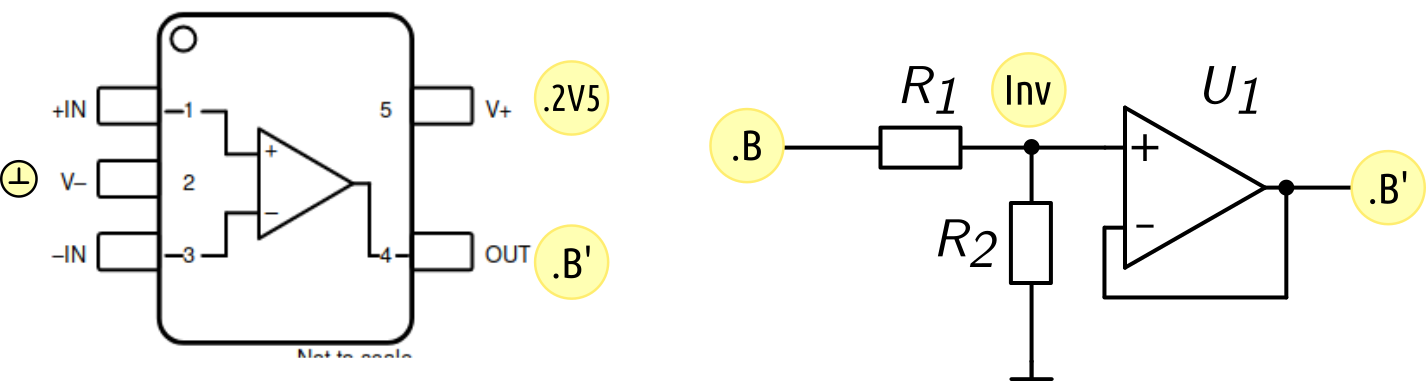
\includegraphics[width=1.0\textwidth]{PO/SV/SV}
    % \caption{SI - schematic, n = 1,2}
\end{figure}
\begin{table}[H]
    \centering
    \begin{threeparttable}[b]
        \begin{tabularx}{\linewidth}{ >
                    {\hsize=.25\hsize}X >
                    {\hsize=0.5\hsize}X >
                    {\hsize=.25\hsize}X  >
                    {\hsize=.5\hsize}X >
                    {\hsize=.25\hsize}X  >
                    {\hsize=3\hsize}X
            }
                  & \multicolumn{4}{c}{pin} &                                                         \\
            \cmidrule(lr){3-6}
            Id    & Net                     & Nb. & Name         & Type             & Function        \\
            \midrule
            $U_1$ & Inv                     & 1   & \texttt{+IN} & \leftsquigarrow  & input           \\
            $U_1$ & \Gnd                    & 2   & \texttt{V-}  & \Gnd             &                 \\
            $U_1$ & .B'                     & 3   & \texttt{-IN} & \leftsquigarrow  & inverting input \\
            $U_1$ & .B'                     & 4   & \texttt{OUT} & \rightsquigarrow & output          \\
            $U_1$ & .2V5                    & 5   & \texttt{V+}  & \leftarrow       & power supply    \\
            $R_1$ & .B                      & 1   & \texttt{OUT} &                  &                 \\
            $R_1$ & Inv                     & 2   & \texttt{OUT} &                  &                 \\
            $R_2$ & Inv                     & 1   & \texttt{OUT} &                  &                 \\
            $R_2$ & \Gnd                    & 2   & \texttt{OUT} &                  &                 \\
        \end{tabularx}
    \end{threeparttable}
    %  \caption{WD - Pin mapping}
\end{table}

\begin{table}[H]
    \centering
    \begin{threeparttable}[b]
        \begin{tabularx}{\linewidth}{
                >{\hsize=0.25\hsize}X
                >{\hsize=0.75\hsize}X
                >{\hsize=1.5\hsize}X
                >{\hsize=0.5\hsize}X
                >{\hsize=2\hsize}X}
            \toprule
            Id    & Desc                       & Order Code           & Package & Note                                           \\
            \midrule
            $U_1$ & \cite{ti_opax391_2022}     & OPA391DCKR/931       & SC70-5  &                                                \\
            $R_1$ & \SI{129}{\kilo\ohm}        & RN73H2ATTD1293B25/52 & 0603    & \cite{noauthor_rn73h_2022}, \SI{0.1}{\percent} \\
            $R_2$ & \SI{200}{\kilo\ohm}        & RN73H1JTTD5693B50/59 & 0603    & \cite{noauthor_type_2016} , \SI{0.1}{\percent} \\
            $C_b$ & \SI{100}{\nF}, \SI{16}{\V} & generic              & 0402    & bypass cap                                     \\
            \bottomrule
        \end{tabularx}
    \end{threeparttable}
    \caption{SV - BOM}
    \label{table:wd1}
\end{table}
\input{hardware/modules/PO/SV/SV_issues}
